\subsection{Tageb"ucher}
\subsubsection{Tagebuch eines 1. Semesters\ldots}

\begin{description}
\item[05:30] Der Quarz-Uhr-Timer mit Digitalanzeige gibt ein zaghaftes "`Piep-Piep"'
von sich. Bevor sich dieses zu energischem Gezwitscher entwickelt, sofort
ausgemacht, aus dem Bett geh"upft. F"unf Kilometer Jogging an der Oker,
mit einem Besoffenen zusammengesto"sen, anschlie"send eiskalt geduscht.
\item[06:00] Beim Fr"uhst"uck Heise-Online studiert und dabei neueste Patches geladen.
Danach kritischer Blick in den Spiegel, Outfit genehmigt.
\item[07:00] Zur Uni gehetzt. PK 2.2 erreicht. Pech gehabt: erste Reihe schon besetzt.
Niederschmetternd. Beschlossen, morgen doch noch eher aufzustehen.
\item[07:30] Vorlesung, Algorithmen und Datenstrukturen bei Struckmann. Keine Disziplin!
Einige Kommilitonen lesen
Sportteil der BZ oder gehen ins "`Viertel Nach"' fr"uhst"ucken. Alles
mitgeschrieben. F"uller leer, aber "uber die Witzchen des Dozenten mitgelacht.
\item[08:00] Vorlesung, Lineare Algebra, Marten. Verdammt! Extra neongr"unen Pulli
angezogen und trotz eifrigem Fingerschnippens nicht drangekommen.
\item[10:45] N"achste Vorlesung. Nachbar verl"a"st mit Bemerkung "`Sinnlose
Veranstaltung"' den Raum. Habe mich f"ur ihn beim Prof. entschuldigt.
\item[12:00] Mensa Essen II. Nur unter gr"o"sten Schwierigkeiten
weitergearbeitet, da in der Mensa zu laut.
\item[12:45] In Fachschaft gewesen. Mathe Skript immer noch nicht fertig. Wollte
mich beim Vorgesetzten beschweren. Keinen Termin bekommen. Daran geht die
Welt zugrunde.
\item[13:00] F"unf Leute aus meiner Stuko-Gruppe getroffen. Gleich f"ur drei AG's zur
Klausurvorbereitung verabredet.
\item[13:30] Dreiviertelstunde im Copyshop gewesen und die Klausuren der letzten 10
Jahre mit L"osungen kopiert. Dann Kleine "Ubung: "Altere Semester haben keine
Ahnung.
\item[15:30] In der Bibliothek mit den anderen gewesen. Durfte aber statt der
dringend ben"otigen 18 B"ucher nur vier mitnehmen.
\item[16:00] Gro"se "Ubung. War gut vorbereitet. Hinterher den Assi "uber seine
Irrt"umer aufgekl"art.
\item[18:30] Anhand einschl"agiger Quellen die Promotionsbedingungen eingesehen und
erste Kontakte gekn"upft.
\item[19:45] Abendessen. Verabredung im "`Dialog"' abgesagt. Daf"ur Vorlesungen
der letzten paar Tage nachgearbeitet.
\item[23:00] Videoaufzeichnung von "`Relationale Datenbanken 1"' angesehen und im Bett noch den "`Cormen"'
gelesen. Festgestellt, 18-Stunden-Tag zu kurz. Werde demn"achst die Nacht
hinzunehmen.
\end{description}
\begin{center}
  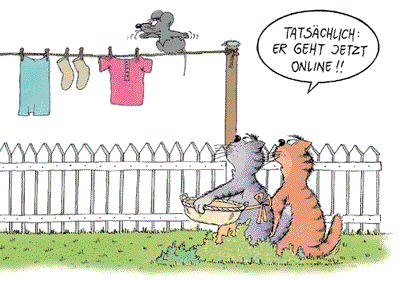
\includegraphics[width=\linewidth]{bilder/comics/stein1.png}
\end{center}
\newpage
\subsubsection{Tagebuch eines 11. Semesters\ldots}

\begin{description}
\item[10.30] Aufgewacht! Ach, Kopfschmerzen, "Ubelkeit, zu deutsch: KATER!
\item[10.45] Der linke gro"se Zeh wird Freiwilliger bei der Zimmertemperaturpr"ufung.
(Arrgh!) Zeh zur"uck. Rechts Wand, links kalt; Mist, bin gefangen.
\item[11.00] Kampf mit dem inneren Schweinehund: Aufstehen oder nicht - das ist
hier die Frage.
\item[11.30] Schweinehund schwer angeschlagen, wende Verz"ogerungstaktik an und
schalte Fernseher ein (inzwischen auch schon verkabelt).
\item[12.05] Mittagsmagazin beginnt. Originalton Moderator: "`Guten Tag liebe
Zuschauer Guten MORGEN liebe Studenten."' Auf die Provokation hereingefallen
und aufgestanden.
\item[13.30] In der Cafeteria der Mensa Katharienstra"se beim Skat mein Mittagessen
verspielt.
\item[14.30] Im Hermanns hereingeschaut. Geld gepumpt und 'ne Kleinigkeit
gegessen: Bier schmeckt wieder! Kurze Diskussion mit ein paar Leuten "uber
die letzte Entwicklung im Computerspielemarkt.
\item[15.45] Kurz in der Bibliothek gewesen. Nix wie raus, total von Erstsemestern
"uberf"ullt.
\item[16.00] F"unf Minuten im IZ gewesen. Nichts los! Keine Zeitung, keine
Flugbl"atter - nichts wie weg.
\item[17.00] Stammkneipe hat immer noch nicht ge"offnet.
\item[18.15] Wichtiger Termin zuhause: Star Trek!
\item[18:20] Mist! Kein Star Trek! Stattdessen Live-"Ubertragung von Barbara Salesh.
SAT 1 war auch schon besser\ldots
\item[19.10] Komme zu sp"at zum Date mit der blonden Erstsemesterin im Eusebia.
Immer dieser Stre"s!
\item[01.00] Die Kneipen schlie"sen auch schon immer fr"uher\ldots Umzug ins Jolly Joker.
\item[04.20] Tagespensum erf"ullt. Das Bett lockt.
\item[05.35] Am Okerufer von Erstsemester "uber'n Haufen gerannt worden. Hat mich
gemein beschimpft.
\item[06.45] Bude m"uhevoll erreicht. Insgesamt \EUR{27,50} ausgegeben. Mehr hatte die
Kleine nicht dabei.
\item[07.05] Schlucke schnell noch ein paar Alkas und schalte kurz das Radio ein.
Stimme des Sprechers: "`Guten Morgen liebe Zuh"orer, gute NACHT liebe
Studenten."'
\end{description}
